%
% design.tex
%
% Copyright (C) 2021 by SpaceLab.
%
% FloripaSat-2 Documentation
%
% This work is licensed under the Creative Commons Attribution-ShareAlike 4.0
% International License. To view a copy of this license,
% visit http://creativecommons.org/licenses/by-sa/4.0/.
%

%
% \brief Design description chapter.
%
% \author Gabriel Mariano Marcelino <gabriel.mm8@gmail.com>
%
% \institution Universidade Federal de Santa Catarina (UFSC)
%
% \version 0.9.0
%
% \date 2021/07/15
%

\chapter{Design Description} \label{ch:design}

.

\section{General Diagrams}

The CubeSat's subsystems are positioned in the 2U physical structure as exemplified in \autoref{fig:subsystems-positioning}. An exploded 3D view of the satellite is showed in \autoref{fig:exploded-view}.

\begin{figure}[!ht]
    \begin{center}
        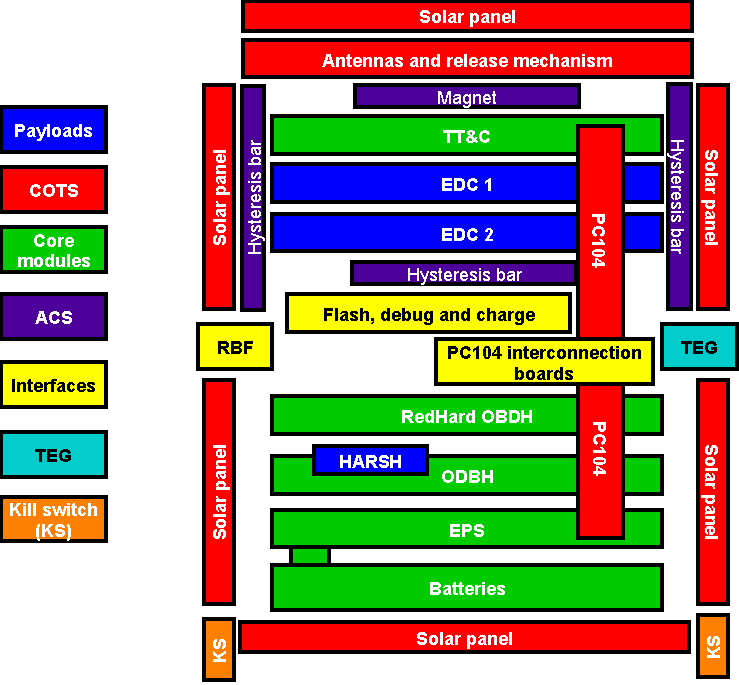
\includegraphics[width=0.7\textwidth]{figures/subsystems-positioning.pdf}
        \caption{Subsystems positioning.}
        \label{fig:subsystems-positioning}
    \end{center}
\end{figure}

\subsection{Power Diagram}

In \autoref{fig:power-diagram} is presented a block diagram showing the satellite's power buses.
The EPS module distributes these buses and have the hability to turn on and off some subsystems, while other modules also have direct control over some dc regulators\cite{eps2}.
The bus used for the antenna module is only active during its deployment. 
The current values showed are the maximum capability and not the nominal operating values, these are determined by the variable power generation of the solar panels as well the loads present in a given time of the satellite's operation.
% TBD
% In \autoref{power-budget} the power consumption of the satellite in showed in detail.

\begin{figure}[!ht]
    \begin{center}
        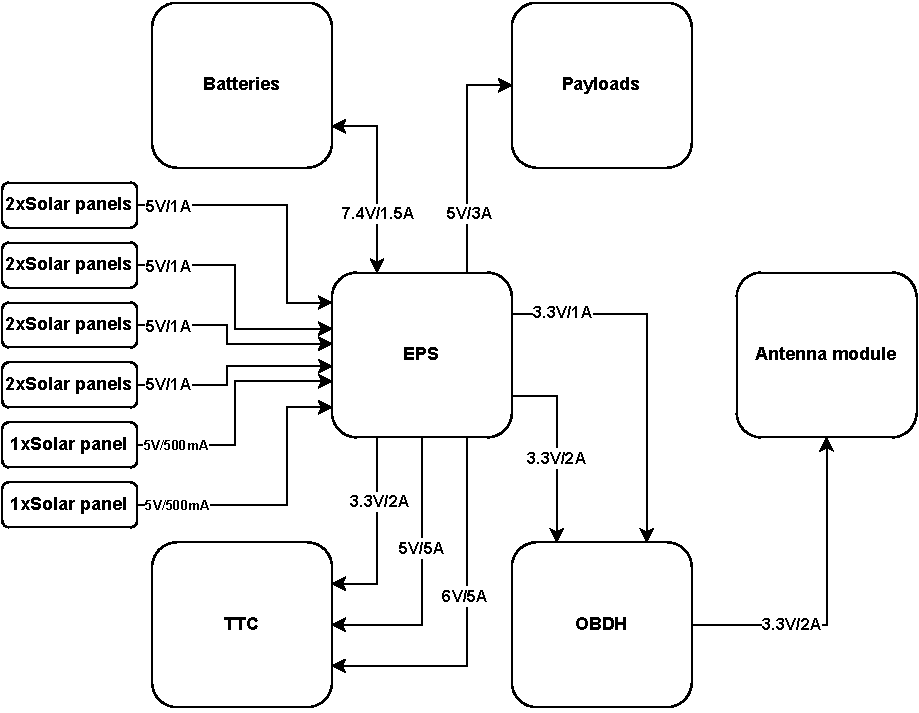
\includegraphics[width=\textwidth]{figures/power_diagram.pdf}
        \caption{Power diagram.}
        \label{fig:power-diagram}
    \end{center}
\end{figure}

%   TBD 
%   In \autoref{fig:datapath-diagram} there is a block diagram showing the satellite modules and the internal communication interfaces.

\subsection{Data Path Diagram}

\begin{figure}[!ht]
    \begin{center}
        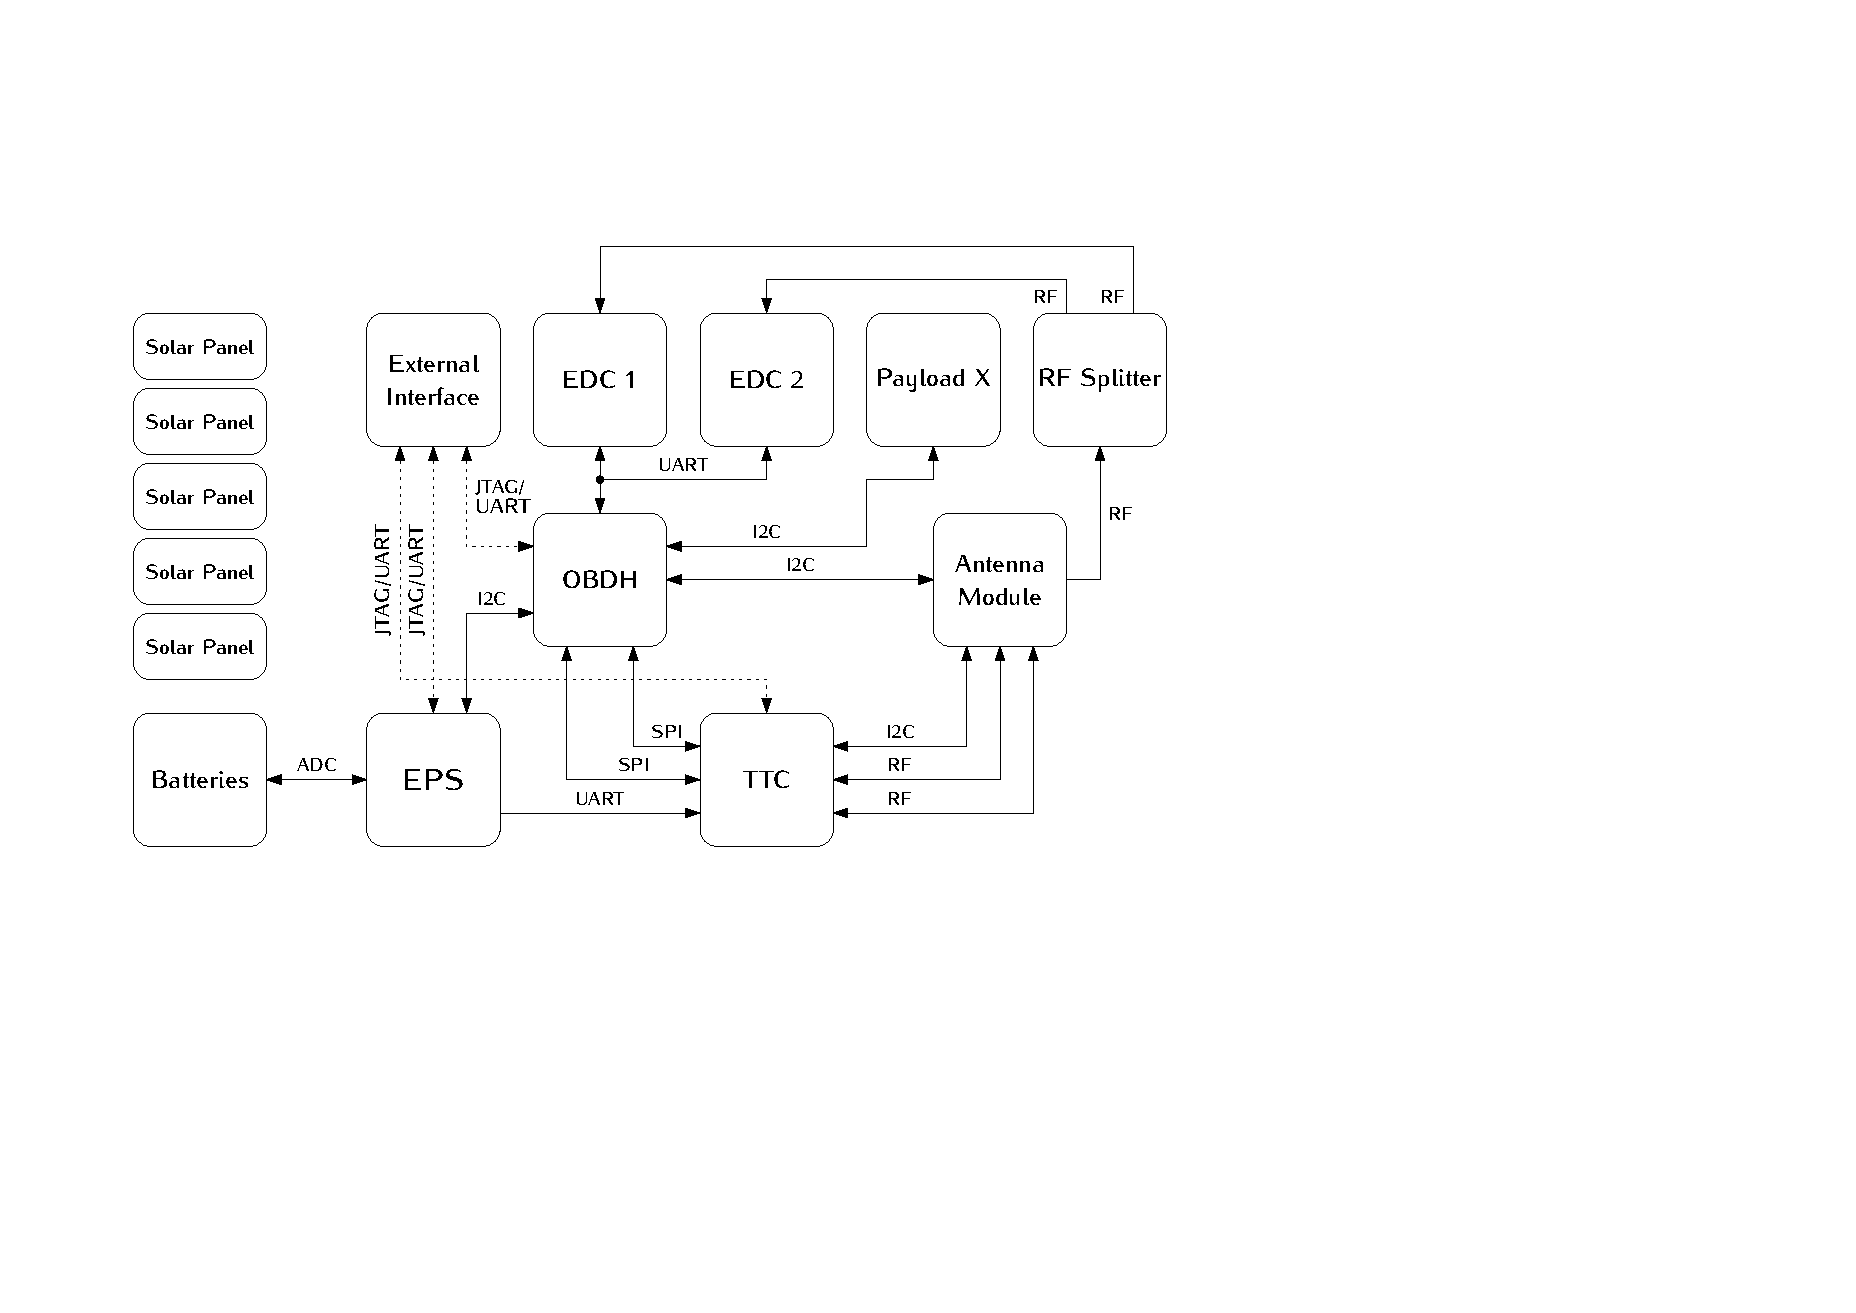
\includegraphics[width=\textwidth]{figures/data_path_diagram.pdf}
        \caption{Data path diagram.}
        \label{fig:data-path}
    \end{center}
\end{figure}

\subsection{Deployment Sequence}

The deployment sequence of the satellite is the routine to be executed just after the launch. The main objective of this operation is to the deploy the antennas and prepare the satellite to start its normal operation.

Just after the satellite is ejected from the deployer, the kill-switches enables the electric power and the three core modules execute the boot sequence (EPS, OBDH and TTC). The EPS module is ready to operate when the boot finishes. The OBDH and the TTC modules waits for a determined period before starting the normal execution.

As the OBDH and the TTC have access to the antenna module, both subsystem can control the deployment of the antennas. Following the CDS\nomenclature{\textbf{CDS}}{\textit{CubeSat Design Specification.}} specifications \cite{cds}, all CubeSats must wait 30 minutes to deploy the antennas and 45 minutes to transmit any RF signal. This way, the OBDH waits 45 minutes to send the deployment command to the antenna module. As redundancy, the TTC waits 55 minutes to execute the same operation.

The \autoref{fig:deployment-flowchart} has a flowchart that illustrates the deployment sequence of the service modules.

\begin{figure}[!ht]
    \begin{center}
        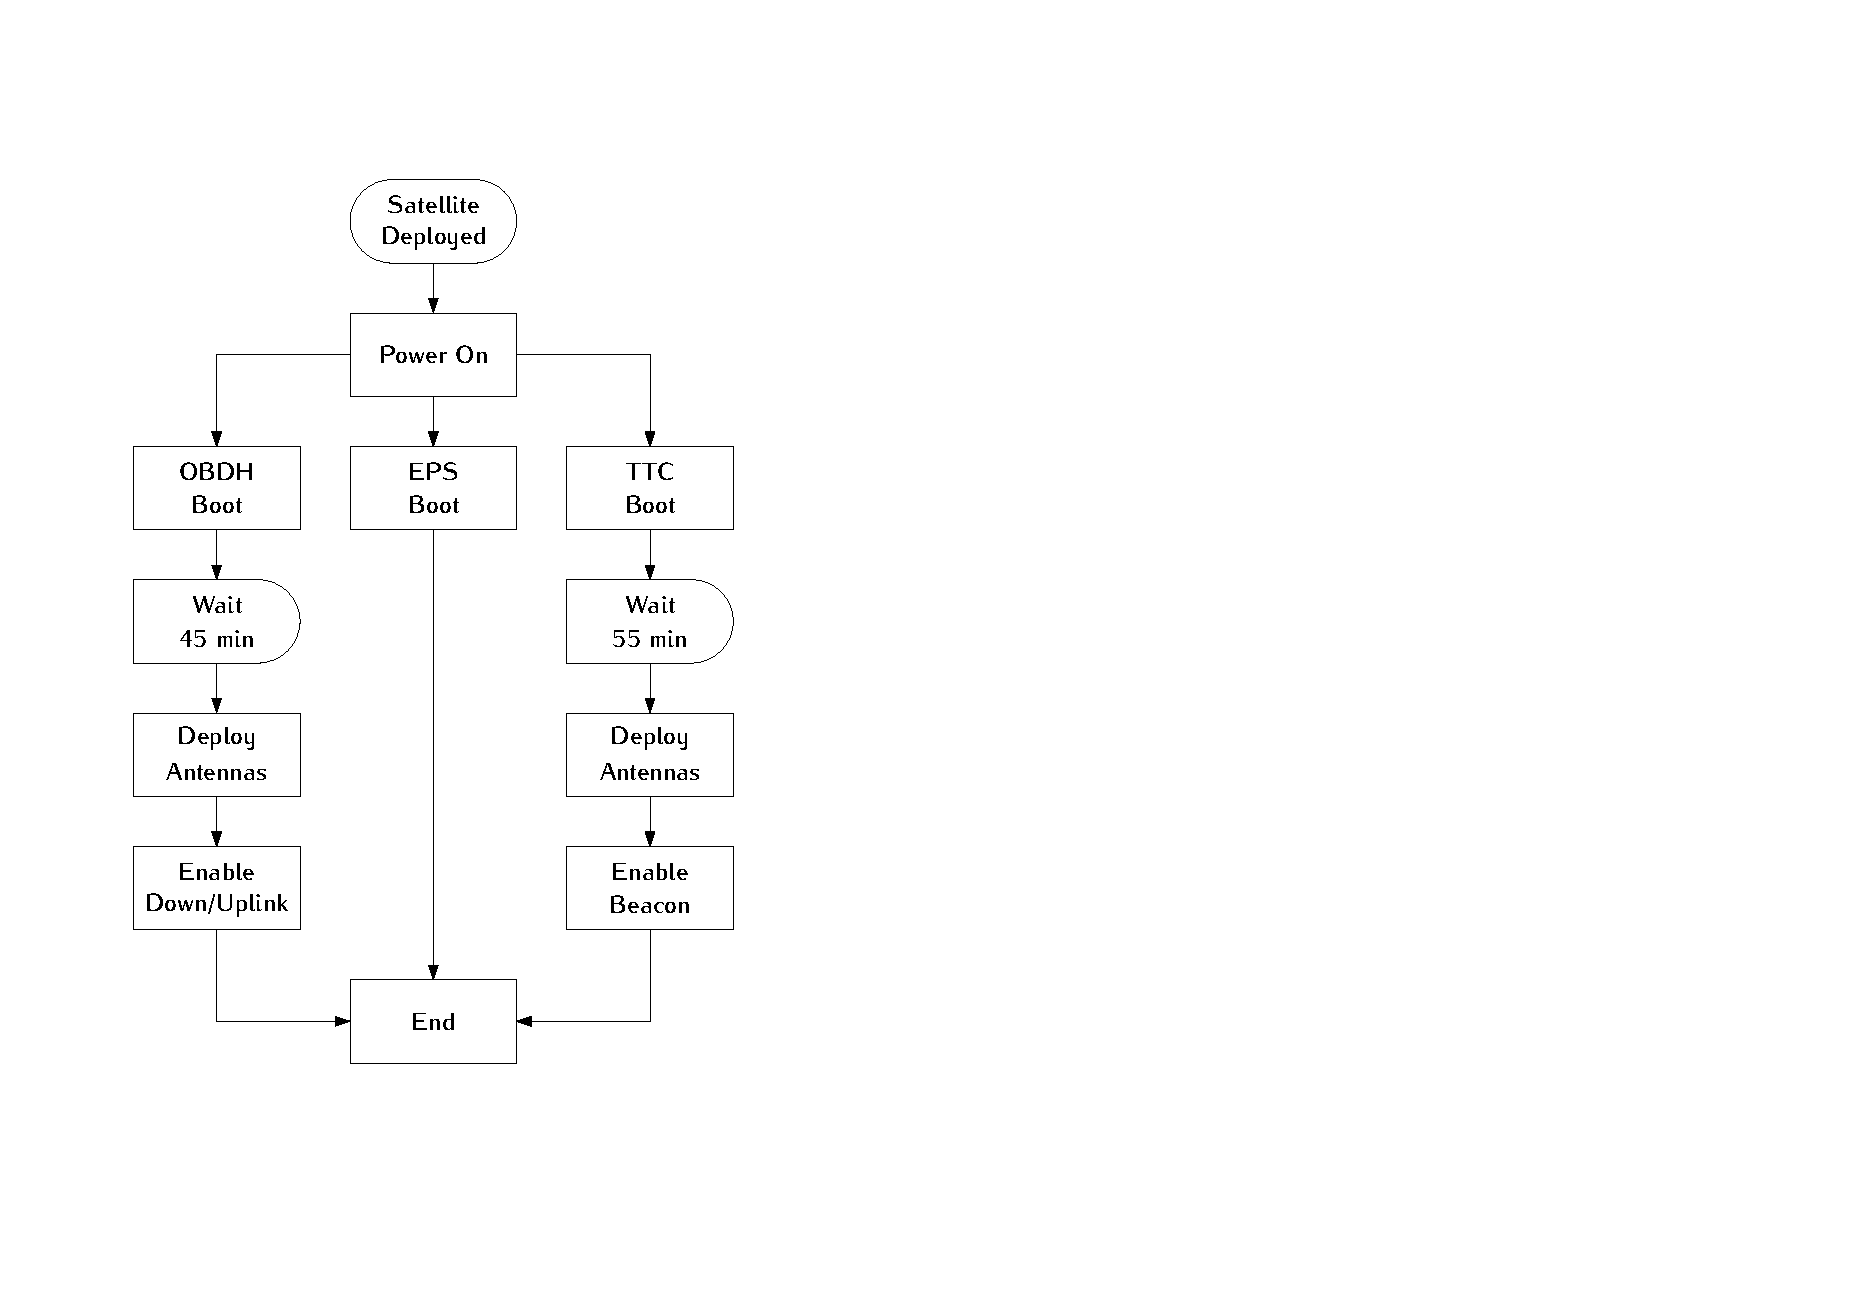
\includegraphics[width=0.5\textwidth]{figures/deployment-flowchart.pdf}
        \caption{Flowchart of the deployment sequence.}
        \label{fig:deployment-flowchart}
    \end{center}
\end{figure}

\subsection{Beacon Operation}

After the boot sequence of the beacon microcontroller, the operation of the beacon starts. The normal operation consist on reading the data from the EPS and the TTC modules, transmit the valid data (EPS or TTC package, in this order of priority), wait 60 seconds and repeat this sequence. The \autoref{fig:beacon-flowchart} has a flowchart of this behaviour.

\begin{figure}[!ht]
    \begin{center}
        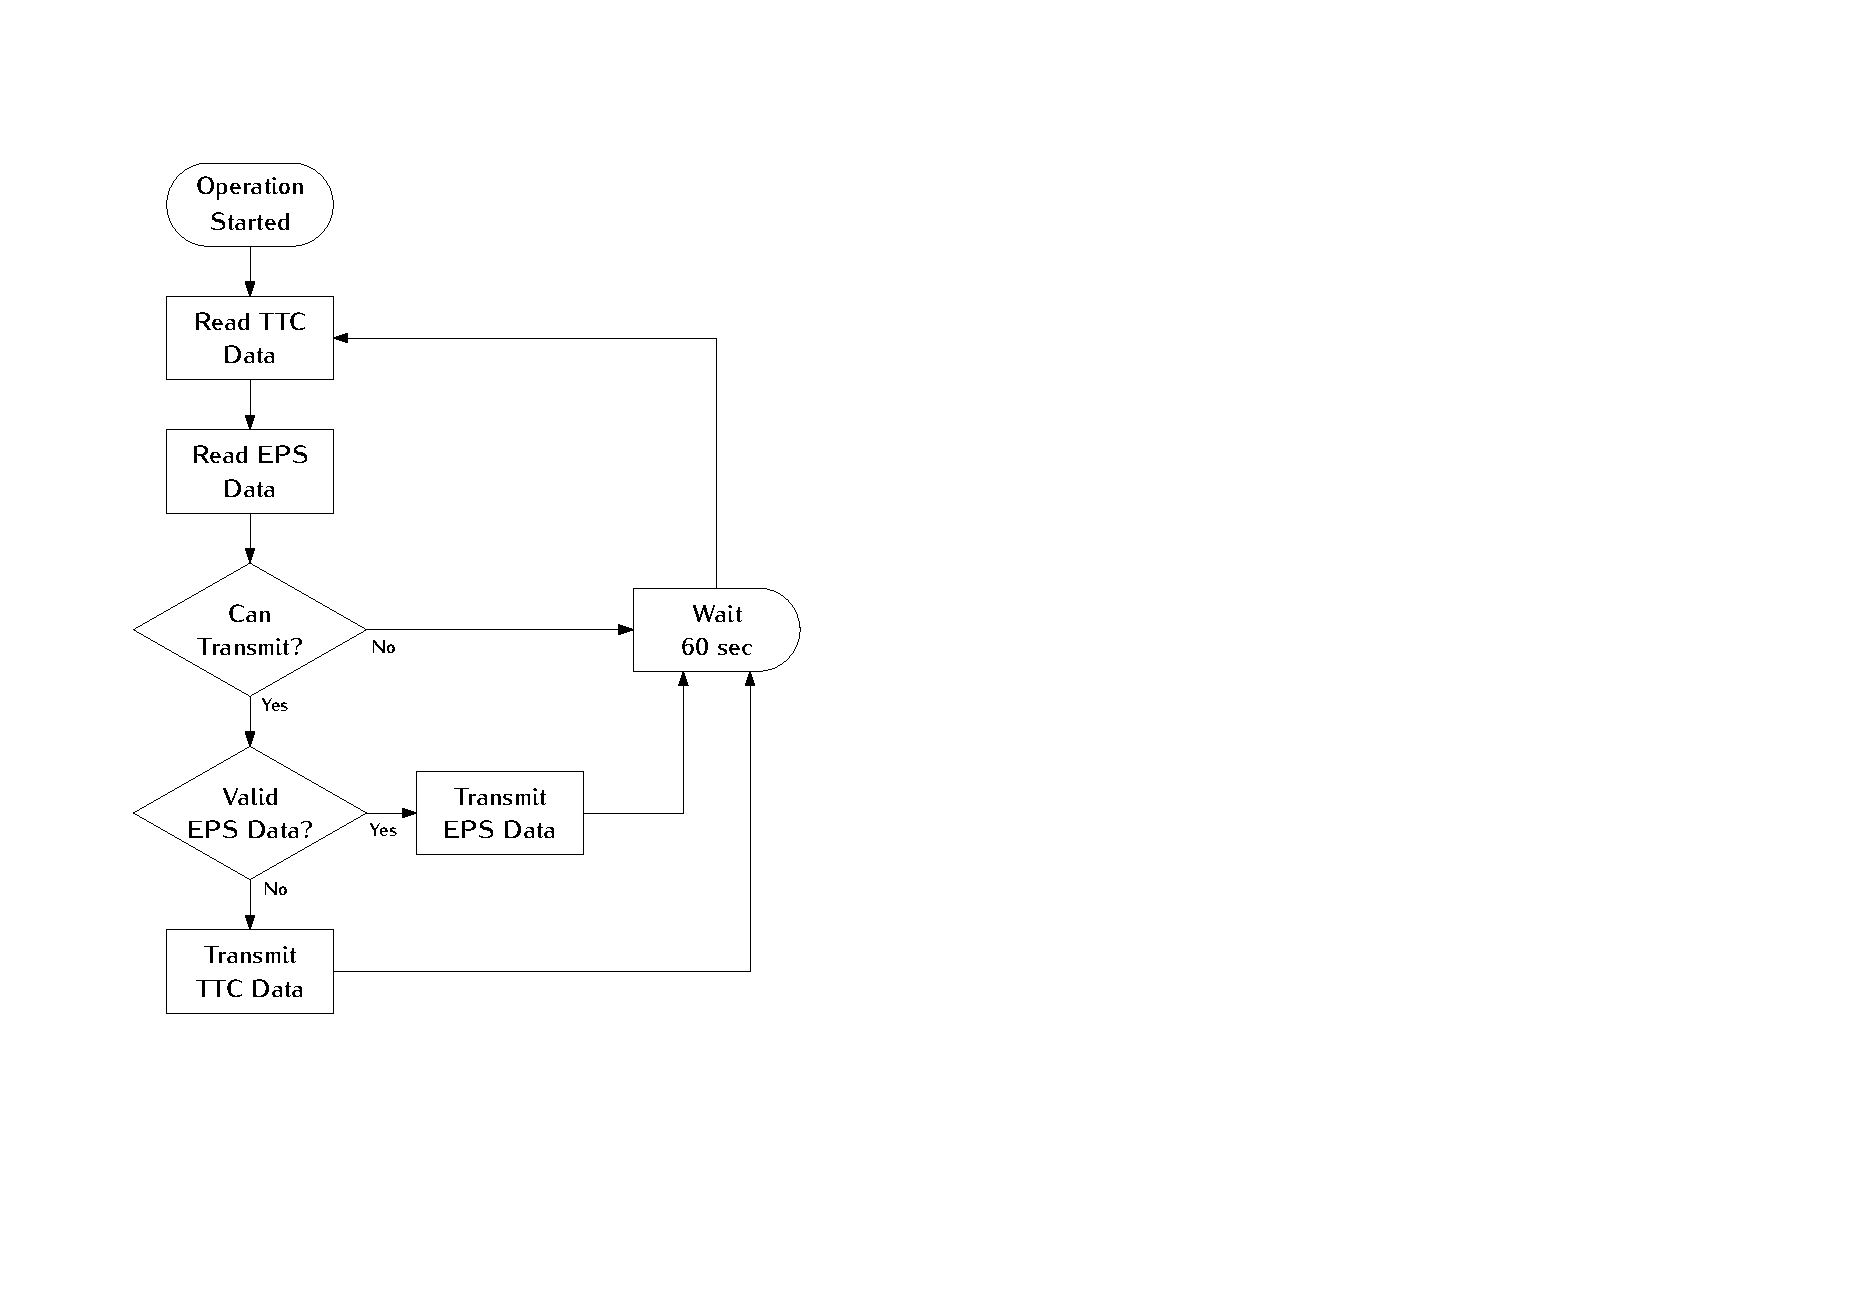
\includegraphics[width=0.55\textwidth]{figures/beacon-flowchart.pdf}
        \caption{Flowchart of the normal beacon operation.}
        \label{fig:beacon-flowchart}
    \end{center}
\end{figure}

\subsection{OBDH Operation}

After the boot sequence of the OBDH microcontroller, the operation of the OBDH starts. The normal operation consist on reading the housekeeping data from the EPS, TTC, payloads, antenna module and the OBDH (its own housekeeping data), save the read data on the non-volatile memory and transmit the housekeeping data of the satellite as a beacon. After that, it waits 60 seconds and check if a new telecommand was received, if true process the telecommand, if not, does nothing. After this sequence, these steps start again. The \autoref{fig:obdh-flowchart} has a flowchart of this behaviour.

\begin{figure}[!ht]
    \begin{center}
        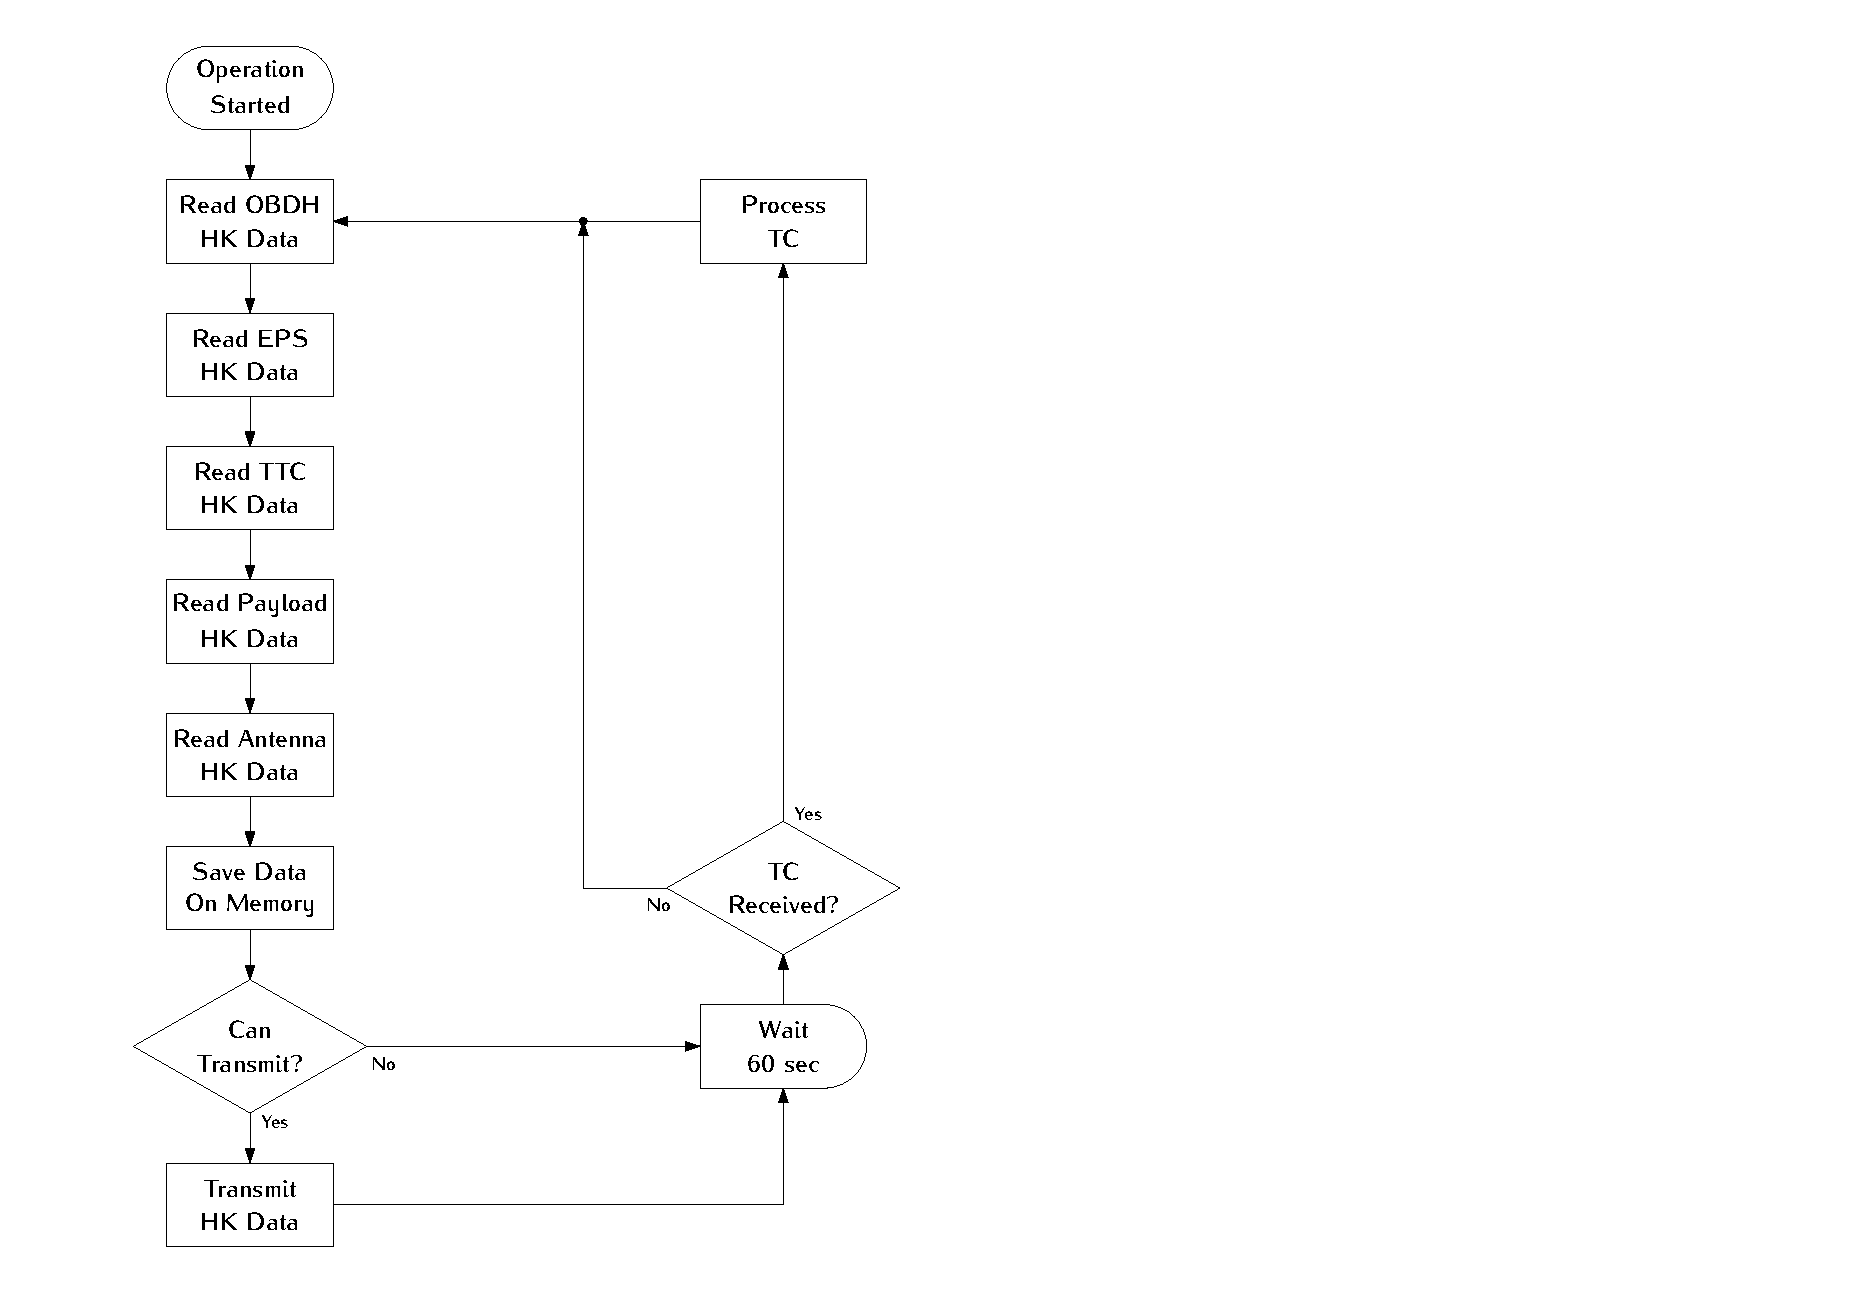
\includegraphics[width=0.63\textwidth]{figures/obdh-flowchart.pdf}
        \caption{Flowchart of the normal OBDH operation.}
        \label{fig:obdh-flowchart}
    \end{center}
\end{figure}

\subsubsection{Telecommand Processing}

.

\begin{figure}[!ht]
    \begin{center}
        \includegraphics[width=0.8\textwidth]{figures/tc-flowchart.pdf}
        \caption{Flowchart of telecommand processing.}
        \label{fig:tc-flowchart}
    \end{center}
\end{figure}

\subsection{EPS Operation}

The operation of the EPS microcontroller starts shortly after the release of the CubeSat in its orbit by the deployer.
In the first 60 minutes the module operation consist of reading the housekeeping data from its sensors and managing the duty cycles of the MPPT and heaters.
When operational, the TTC and OBDH modules send separete periodic requests to the EPS for fowarding the housekeeping data acquired.
The TTC receives a simplifed version while the OBDH receives a complete version of the data.
The \autoref{fig:eps-flowchart} has a flowchart of this behaviour.

\begin{figure}[!ht]
    \begin{center}
        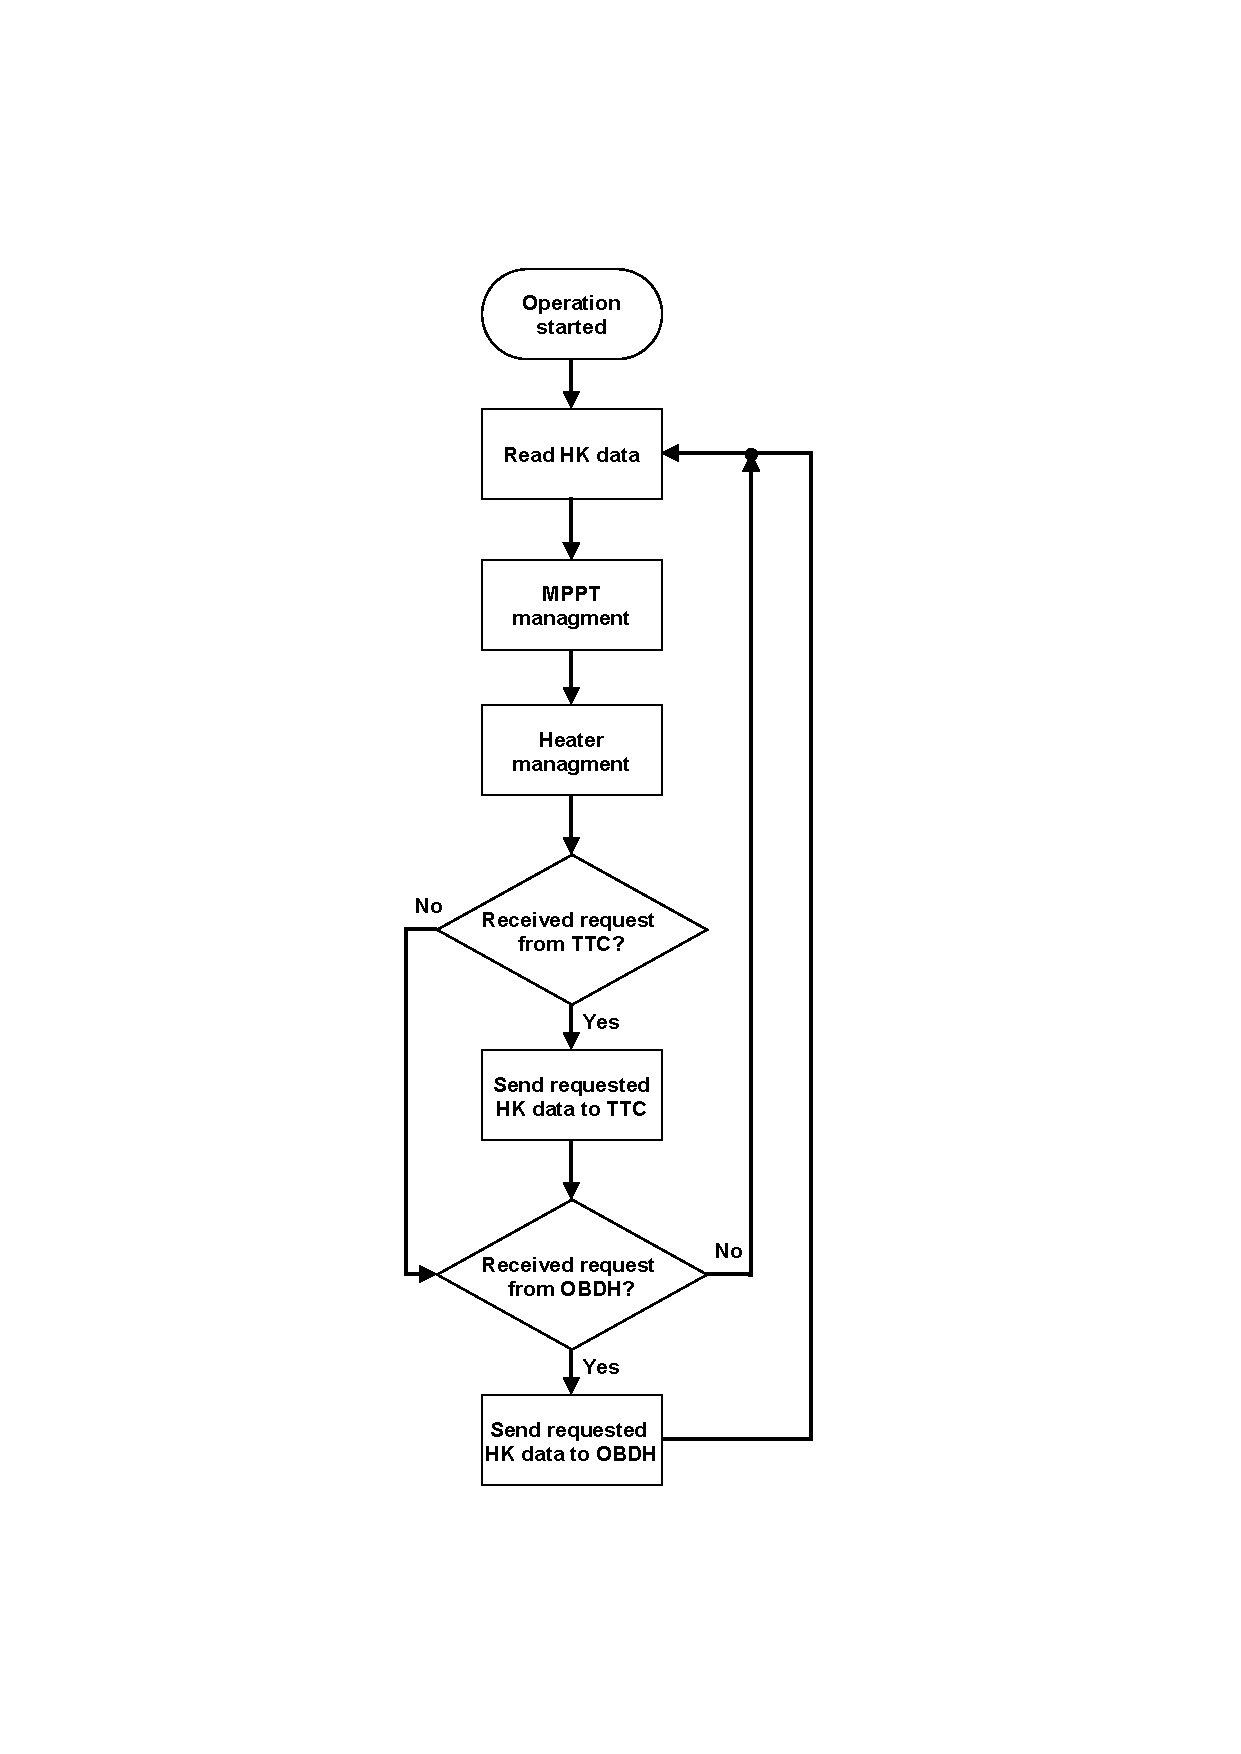
\includegraphics[width=0.45\textwidth]{figures/eps_flowchart.pdf}
        \caption{Flowchart of the normal EPS operation.}
        \label{fig:eps-flowchart}
    \end{center}
\end{figure}

\section{General Behaviour}

.

\section{PC-104 Bus}

\subsection{Interface}

To electrically connect all the satellite modules, a PC-104 bus standard is being used. This bus is composed by 104 lines disposed by four rows of 26 pins each (with a vertical and horizontal pitch of 2,54 mm).

Using the \autoref{fig:pc104-ref-diagram} as reference, all used positions and signals of the PC-104 bus are presented in \autoref{tab:pc104-pinout}. The \autoref{tab:pc104-signals} describes each signal and which modules are connected to them.

\begin{figure}[!ht]
    \begin{center}
        \includegraphics[width=0.5\textwidth]{figures/pc104-diagram}
        \caption{Reference diagram of the PC-104 bus (top view of a generic module).}
        \label{fig:pc104-ref-diagram}
    \end{center}
\end{figure}

\begin{table}[!h]
    \centering
    \begin{tabular}{cllll}
        \toprule[1.5pt]
        \textbf{Pin Row}   & \textbf{H1 Odd}  & \textbf{H1 Even} & \textbf{H2 Odd} & \textbf{H2 Even} \\
        \midrule
        1-2                & -                & -                & -               & -                \\
        3-4                & -                & -                & EDC\_1\_EN      & EDC\_2\_EN       \\
        5-6                & -                & -                & BE\_UART\_RX    & -                \\
        7-8                & RA\_GPIO\_0      & RA\_GPIO\_1      & BE\_UART\_TX    & GPIO\_0          \\
        9-10               & RA\_GPIO\_2      & BE\_EN           & -               & -                \\
        11-12              & RA\_RESET        & RA\_EN           & BE\_SPI\_MOSI   & BE\_SPI\_CLK     \\
        13-14              & -                & -                & BE\_SPI\_CS     & BE\_SPI\_MISO    \\
        15-16              & -                & -                & -               & -                \\
        17-18              & EDC\_UART\_RX/TX & PLX\_EN          & -               & GPIO\_1          \\
        19-20              & EDC\_UART\_TX/RX & GPIO\_2          & -               & GPIO\_3          \\
        21-22              & -                & -                & -               & GPIO\_4          \\
        23-24              & -                & -                & -               & -                \\
        25-26              & -                & -                & PL\_VCC         & PL\_VCC          \\
        27-28              & -                & -                & TTC\_VCC        & TTC\_VCC         \\
        29-30              & GND              & GND              & GND             & GND              \\
        31-32              & GND              & GND              & GND             & GND              \\
        33-34              & -                & -                & -               & -                \\
        35-36              & RA\_SPI\_CLK     & -                & ANT\_VCC        & ANT\_VCC         \\
        37-38              & RA\_SPI\_MISO    & -                & -               & -                \\
        39-40              & RA\_SPI\_MOSI    & RA\_SPI\_CS      & -               & -                \\
        41-42              & PL\_I2C\_SDA     & -                & -               & GPIO\_5          \\
        43-44              & PL\_I2C\_SCL     & -                & -               & -                \\
        45-46              & OBDH\_VCC        & OBDH\_VCC        & BAT\_VCC        & BAT\_VCC         \\
        47-48              & PL\_VCC          & PL\_VCC          & -               & -                \\
        49-50              & RA\_VCC          & RA\_VCC          & EPS\_I2C\_SDA   & -                \\
        51-52              & BE\_VCC          & BE\_VCC          & EPS\_I2C\_SCL   & -                \\
        \bottomrule[1.5pt]
    \end{tabular}
    \caption{PC-104 bus pinout.}
    \label{tab:pc104-pinout}
\end{table}

\begin{table}[!h]
    \centering
    \begin{tabular}{lL{0.18\textwidth}L{0.17\textwidth}L{0.33\textwidth}}
        \toprule[1.5pt]
        \textbf{Signal}  & \textbf{Pin(s)} & \textbf{Used By}     & \textbf{Description} \\
        \midrule
        GND              & H1-29/30/31/32, H2-29/30/31/32 & All   & Ground reference \\
        BAT\_VCC         & H2-45, H2-46    & EPS                  & Battery terminals (+) \\
        ANT\_VCC         & H2-35, H2-36    & EPS, ANT             & Antenna power supply (3.3 V) \\
        OBDH\_VCC        & H1-45, H1-46    & EPS, OBDH            & OBDH power supply (3.3 V) \\
        TTC\_VCC         & H2-27, H2-28    & EPS, TTC             & TTC power supply (3.3 V) \\
        PL\_VCC          & H1-47/48, H2-25/26 & EPS, EDC 1/2, Payload X & Payloads power supply (5 V) \\
        RA\_VCC          & H1-49, H1-50    & EPS, TTC             & Main radio power supply (5 V) \\
        BE\_VCC          & H1-51, H1-52    & EPS, TTC             & Beacon power supply (6 V) \\
        RA\_SPI\_CLK     & H1-35           & OBDH, TTC            & CLK signal of the main radio SPI bus \\
        RA\_SPI\_MISO    & H1-37           & OBDH, TTC            & MISO signal of the main radio SPI bus \\
        RA\_SPI\_MOSI    & H1-39           & OBDH, TTC            & MOS signal of the main radio SPI bus \\
        RA\_SPI\_CS      & H1-40           & OBDH, TTC            & CS signal of the main radio SPI bus \\
        EPS\_I2C\_SDA    & H2-49           & OBDH, EPS            & SDA signal of the EPS I2C bus \\
        EPS\_I2C\_SCL    & H2-51           & OBDH, EPS            & SCL signal of the EPS I2C bus \\
        BE\_UART\_RX     & H2-5            & EPS, TTC             & EPS TX, Beacon RX (UART bus) \\
        BE\_UART\_TX     & H2-7            & EPS, TTC             & EPS RX, Beacon TX (UART bus) \\
        EDC\_UART\_TX/RX & H1-25           & OBDH, EDC 1/2        & OBDH TX, EDCs RX (UART bus) \\
        EDC\_UART\_RX/TX & H1-27           & OBDH, EDC 1/2        & OBDH RX, EDCs TX (UART bus) \\
        BE\_EN           & H1-10           & EPS, TTC             & Beacon radio power enable \\
        RA\_EN           & H1-12           & EPS, OBDH            & Main radio power enable \\
        EDC\_1\_EN       & H2-3            & OBDH, EDC 1          & EDC 1 enable signal \\
        EDC\_2\_EN       & H2-4            & OBDH, EDC 2          & EDC 2 enable signal \\
        PLX\_EN          & H1-18           & OBDH, Payload X      & Payload X enable (GPIO) \\
        PL\_I2C\_SDA     & H1-41           & OBDH, Payload X      & SDA signal of the payload I2C bus \\
        PL\_I2C\_SCL     & H1-43           & OBDH, Payload X      & SCL signal of the payload I2C bus \\
        GPIO\_N          & H1-20, H2-8/18/20/22/42  & OBDH        & GPIO pin (not used) \\
        \bottomrule[1.5pt]
    \end{tabular}
    \caption{PC-104 bus signal description.}
    \label{tab:pc104-signals}
\end{table}

The distribution pattern of pins adopted in this project is a mix of multiple different patterns from CubeSat modules manufacturers, like GomSpace, ISIS and Endurosat. Some pins are positioned to attend specific project requirements, and it is possible that the adopted pattern is not totally compatible to some commercial modules.

Beyond the PC-104 bus, there are some signals connected directly by wires and cables, like the control and power pins of the antenna module, the battery charger and the programming ports.

\subsection{Form Factor}

The form factor follows a similar specification of the PC-104 standard\cite{pc104-specification}.
The connector used for the interface differs given the module, the isolation heigth and presence of pin or receptable are definied from the overall stack up of the subystems inside the CubeSat 2U structure.
% TBD: include reference to mechanical design here
The core modules have smoothed edges and some linear mounting hole distances different from the standard, these are according to fit in a CubeSat form factor.
The PC-104 form factor used can be seen in \autoref{fig:pc104-form-factor}.

\begin{figure}[!ht]
    \begin{center}
        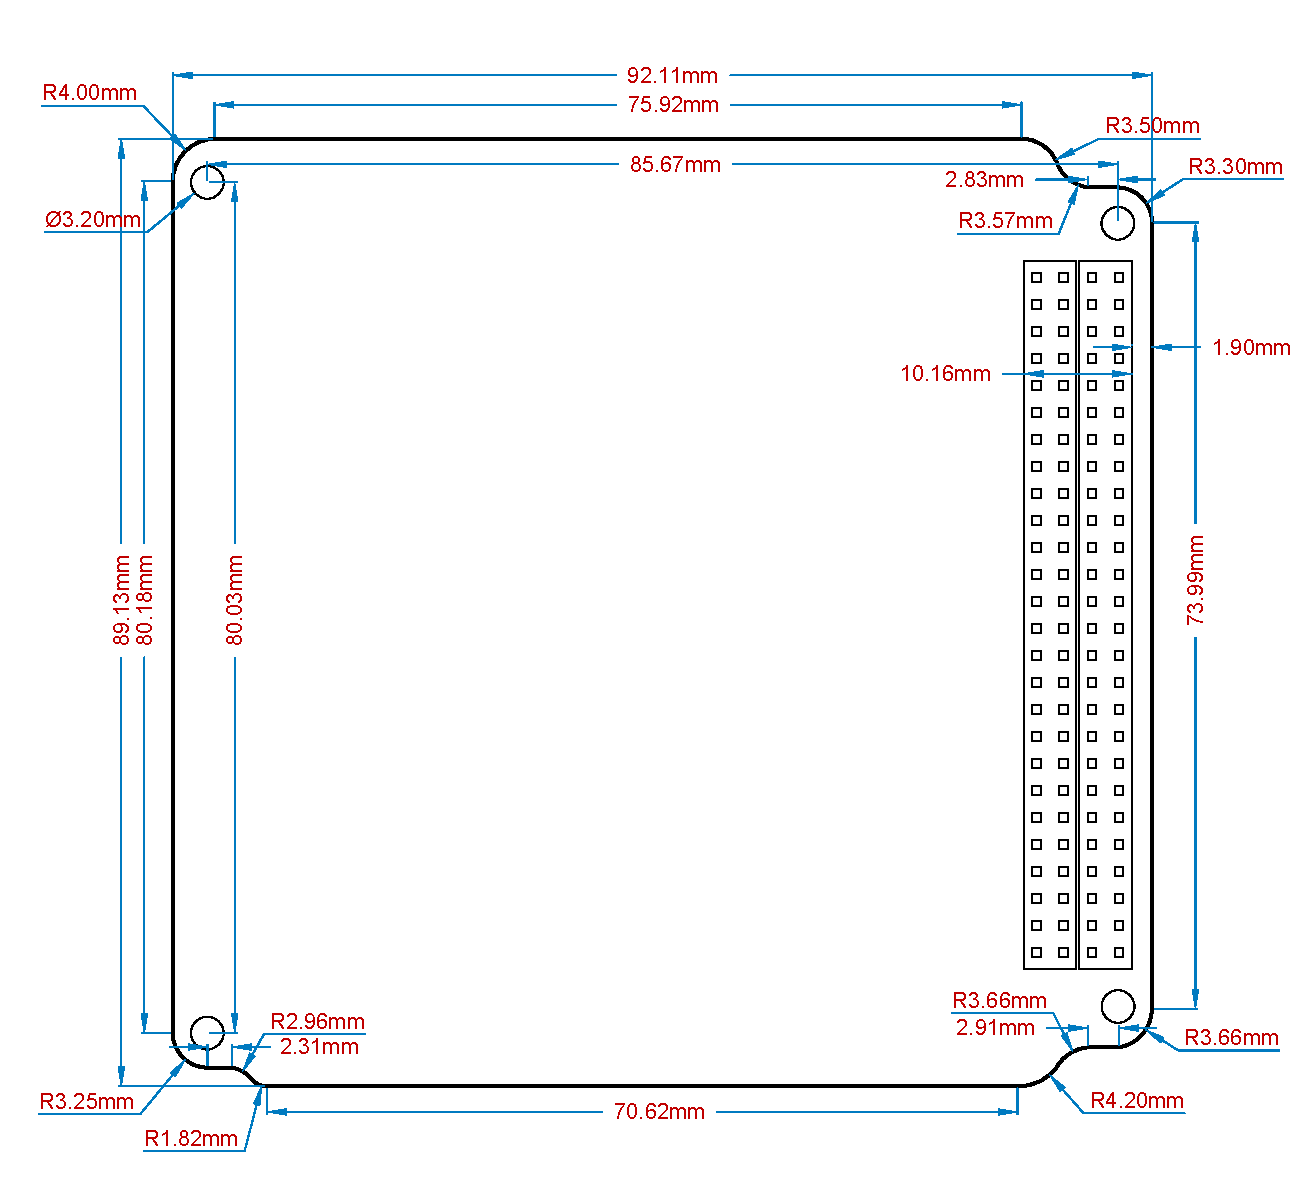
\includegraphics[width=0.75\textwidth]{figures/pc104-form-factor.pdf}
        \caption{PC-104 Form Factor.}
        \label{fig:pc104-form-factor}
    \end{center}
\end{figure}

\section{Telecommunication}

This section describes the configuration and behaviour of the telecommunication subsystems of the satellite. There are three types links available in the CubeSat: beacon, downlink and uplink. The beacon link is a periodic transmission of packets with a basic telemetry data of the satellite (containing data from the EPS or TTC subsystems). The downlink is the link used to receive all data from the satellite, including the results of all experiments, telemetry data and telecommands feedback. And the uplink is used for send telecommands from a ground station to the satellite.

The payload of all packets follows the same structure, with an ID number, the source address (callsign) and the content of the packet (variable according to each type of packet). Following the NGHam protocol characteristics, the maximum length of a packet, including the ID and the source address, is 220 bytes. The \autoref{fig:fsat-pkt-structure} illustrates this packet structure.

\begin{figure}[!ht]
    \begin{center}
        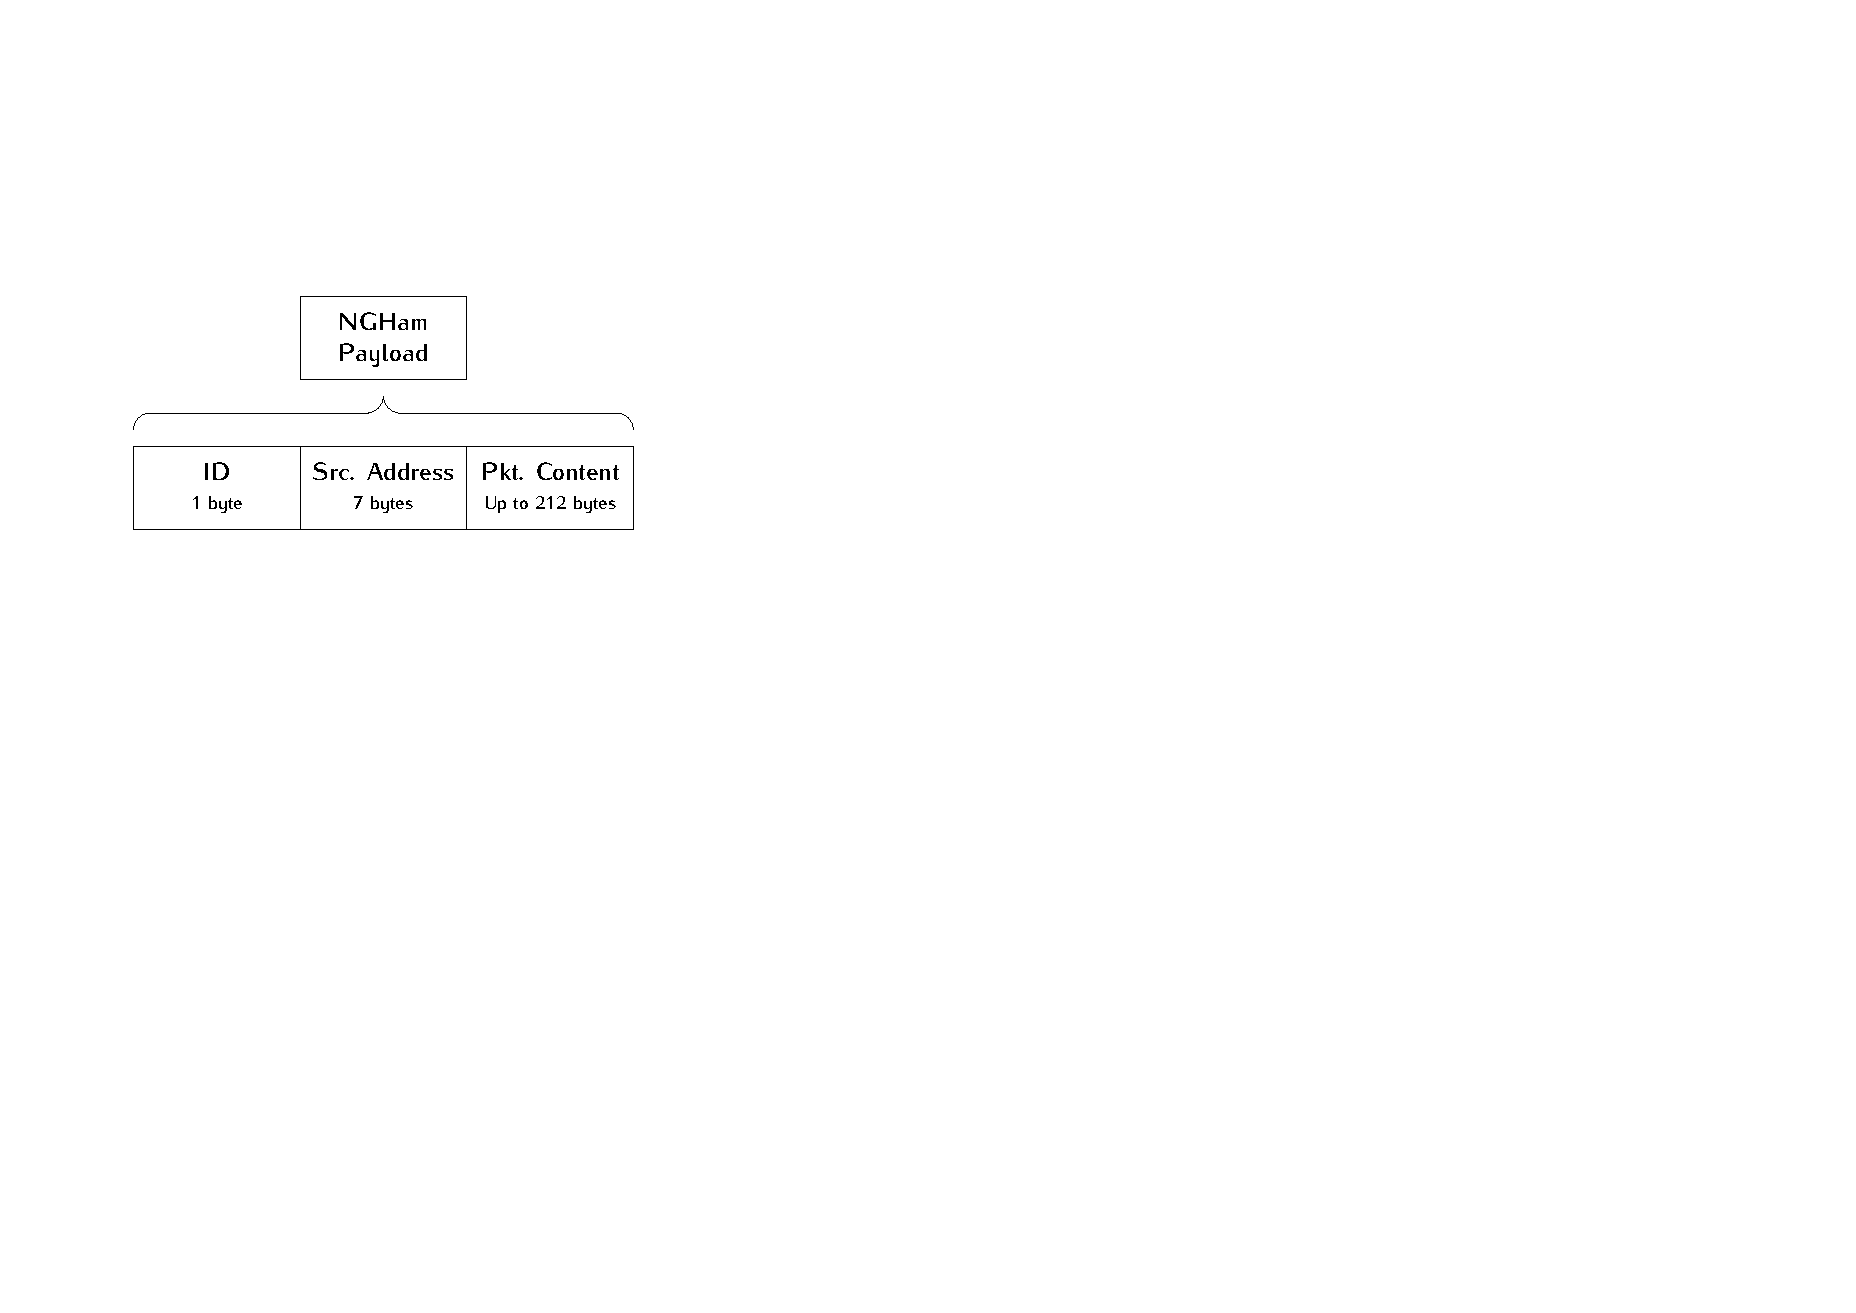
\includegraphics[width=0.5\textwidth]{figures/floripasat-packet-structure.pdf}
        \caption{Payload structure of the FloripaSat-2 packets.}
        \label{fig:fsat-pkt-structure}
    \end{center}
\end{figure}

The \autoref{tab:packets-struct} summarizes all types of packets transmitted or received by the satellite, with the ID number, the structure and length of and the access type of each packet.

\begin{landscape}
    \begin{table}[ht]
        \centering
        \begin{tabular}{llccccc}
            \toprule[1.5pt]
            \multirow{2}{*}{\textbf{Link}} & \multirow{2}{*}{\textbf{Packet Name}} & \multicolumn{4}{c}{\textbf{Payload}} & \multirow{2}{*}{\textbf{Access}} \\
            \cmidrule{3-6}
                                      &                       & \textbf{ID}  & \textbf{Source Callsign}   & \textbf{Data (up to 220 bytes)}            & \textbf{Size (bytes)} & \\
            \midrule
            \multirow{2}{*}{Beacon}   & EPS data              & 00h & \multirow{2}{*}{`` '' + ``PY0EFS''} & EPS data                                   & 46                    & Public \\
                                      & TTC Data              & 01h &                                     & TTC data                                   & 19                    & Public \\
            \midrule
            \multirow{6}{*}{Downlink} & General telemetry     & 20h & \multirow{6}{*}{`` '' + ``PY0EFS''} & OBDH/EPS data                              & 78                    & Public \\
                                      & Ping answer           & 21h &                                     & Requester callsign                         & 15                    & Public \\
                                      & Data request answer   & 22h &                                     & Requester callsign + data ID + ts. + data  & 20 to 220             & Public \\
                                      & Message broadcast     & 23h &                                     & Requester + dst. callsign + message        & 22 to 60              & Public \\
                                      & Payload data          & 24h &                                     & Payload ID + payload data                  & 9 to 220              & Public \\
                                      & TC feedback           & 25h &                                     & Req. callsign + TC packet ID + timestamp   & 20                    & Public \\
            \midrule
            \multirow{12}{*}{Uplink}  & Ping request          & 40h & \multirow{12}{*}{Any Callsign}      & None                                       & 8                     & Public \\
                                      & Data request          & 41h &                                     & Data ID + Start ts. + End ts. + Hash       & 37                    & Private \\
                                      & Broadcast Message     & 42h &                                     & Dst. callsign + message                    & 15 to 53              & Public \\
                                      & Enter hibernation     & 43h &                                     & Hibernation in hours + Hash                & 30                    & Private \\
                                      & Leave hibernation     & 44h &                                     & Hash                                       & 28                    & Private \\
                                      & Activate module       & 45h &                                     & Module ID + Hash                           & 29                    & Private \\
                                      & Deactivate module     & 46h &                                     & Module ID + Hash                           & 29                    & Private \\
                                      & Activate payload      & 47h &                                     & Payload ID + Hash                          & 29                    & Private \\
                                      & Deactivate payload    & 48h &                                     & Payload ID + Hash                          & 29                    & Private \\
                                      & Erase memory          & 49h &                                     & Hash                                       & 28                    & Private \\
                                      & Force reset           & 4Ah &                                     & Hash                                       & 28                    & Private \\
                                      & Get payload data      & 4Bh &                                     & Payload ID + Args. + Hash                  & 41                    & Private \\
            \bottomrule[1.5pt]
        \end{tabular}
        \caption{Telecommunication packets and their content.}
        \label{tab:packets-struct}
    \end{table}
\end{landscape}

The ID of the modules that can be activated or deactivated are available in \autoref{tab:module-id}.

\begin{table}[ht]
    \centering
    \begin{tabular}{lcL{0.53\textwidth}c}
        \toprule[1.5pt]
        \textbf{Module} & \textbf{ID Number} \\
        \midrule
        Battery heater      & 1 \\
        Beacon              & 2 \\
        Periodic telemetry  & 3 \\
        \bottomrule[1.5pt]
    \end{tabular}
    \caption{IDs of the modules that can be activated or deactivated.}
    \label{tab:module-id}
\end{table}

The ID of the payloads, to be used in the activate/deactivate telecommands, are available in \autoref{tab:payload-id}.

\begin{table}[ht]
    \centering
    \begin{tabular}{lc}
        \toprule[1.5pt]
        \textbf{Payload} & \textbf{ID Number} \\
        \midrule
        EDC 1               & 1 \\
        EDC 2               & 2 \\
        Payload-X           & 3 \\
        Radiation monitor   & 4 \\
        \bottomrule[1.5pt]
    \end{tabular}
    \caption{IDs of the payloads.}
    \label{tab:payload-id}
\end{table}

\subsection{Authentication}

All the telecommands classified as private use an HMAC\nomenclature{\textbf{HMAC}}{\textit{Hash-based Message Authenticaion Code.}} authentication scheme. Every type of private telecommand has a unique 16-digit ASCII character key that with the telecommand sequence (or message) generates an 160-bits (20-bytes) hash sequence to be transmitted together with the packet payload. The used hash algorithm is the SHA-1\nomenclature{\textbf{SHA-1}}{\textit{Secure Hash Algorithm 1.}}. The \autoref{fig:hmac-diagram} illustrates this authentication method.

\begin{figure}[!ht]
    \begin{center}
        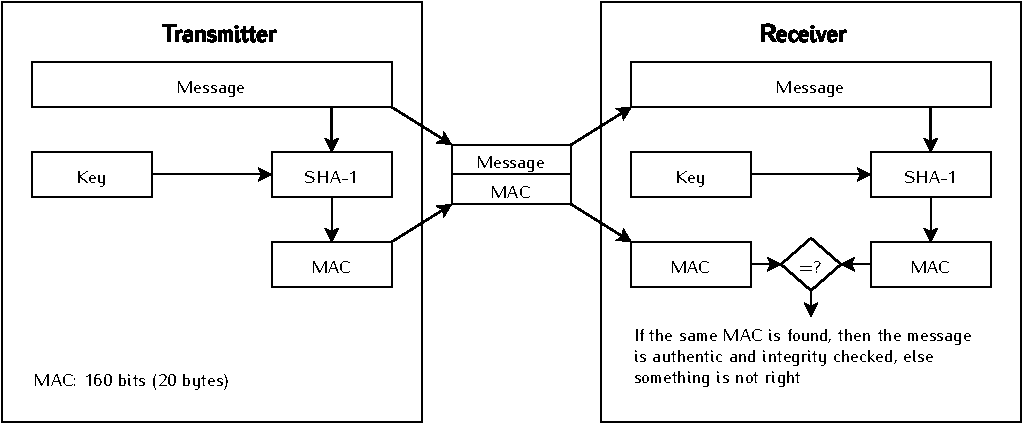
\includegraphics[width=\textwidth]{figures/hmac-diagram.pdf}
        \caption{Diagram of the used HMAC scheme.}
        \label{fig:hmac-diagram}
    \end{center}
\end{figure}

\subsection{Operation Licenses}

.
